%%%%%%%%%%%%%%%%%%%%%%%%%%%           TECHNICAL        %%%%%%%%%%%%%%%%%%%%%%%%%%%%%%%%%%%%%%%%%%

%%%%%%%%%%%%%%%%%%%%%%%%%%             footline             %%%%%%%%%%%%%%%%%%%%%%%%%%%%%%%%%
%\setbeamertemplate{footline}{%
%	\leavevmode%
%	\hbox{%
%		\begin{beamercolorbox}[wd=.126\paperwidth,ht=2.25ex,dp=1ex,right]{footcolor}%      
%			\insertframenumber{} / \inserttotalframenumber\hspace*{5ex}
%	\end{beamercolorbox}}%
%	\vskip0pt%
%}

%%%%%%%%%%%%%%%%%%  page number on the left and logo on the right  %%%%%%%%%%%%%%%%%%%%%%%%%
% \pgfdeclareimage[height=0.8cm]{logo}{zjulogo}
% \logo{\pgfuseimage{logo}{\vspace{-14pt}}}
% %\logo{
\includegraphics[height=0.07\textwidth]{zjulogo.eps}} %这只是我的logo路径
% 
% %页码在左
% \setbeamercolor{footcolor}{fg=black,bg=white} % 设置字体和背景颜色
% \setbeamertemplate{footline}{%
% 	\leavevmode%
% 	\hbox{%
% 		\begin{beamercolorbox}[wd=.126\paperwidth,ht=2.25ex,dp=1ex,right]{footcolor}%      
% 			\insertframenumber{} / \inserttotalframenumber\hspace*{5ex}
% 	\end{beamercolorbox}}%
% 	\vskip0pt%
% }
%%%%%%%%%%  content at every section, highlight current section and hidden other sections  %%%%%
%	\AtBeginSection
%	{
%	\begin{frame}
%	\frametitle{目录}
%	\tableofcontents[currentsection,hideallsubsections]
%	%每一个小节前面都有目录,且高亮当前小节的目录。
%	\end{frame}
%	}
%%%%%%%%%%%%%%%%%%%%%%%%%%%%%%%%%%%%%%%%%%%%%%%%%%%%%%%%%%%%%%%%%%%%%%%%%%%%%%%%%%%%%%%%%%%%%%%

\documentclass[compress]{beamer}

%%%%%%%%%%%%%%%%%%%			加载包
%%%%%%%%%%%%%%%%%%%%%%%%%%%%%%%%%%%%%%%
\usetheme[height=0.8cm]{Rochester}%theme
\useinnertheme[shadow]{rounded} % 设置阴影?
\usepackage[UTF8,noindent]{ctexcap} %noindent阻止段前缩进
\usepackage{graphicx}%插入图片
\usepackage{amsmath} % 插入公式

\mode<presentation>%为了实现分两栏

%为每张PPT插入logo,
% 左下角
%\logo{\makebox[\paperwidth][l]{
\includegraphics[width=1cm,keepaspectratio]{zjulogo.eps}}}
%右下角
\logo{
\includegraphics[width=.8cm,keepaspectratio]{./imags/zjulogo.eps}}


%%%%%%%%%%%%%%%%%%%%%%%%%%%%%%%      setting
%%%%%%%%%%%%%%%%%%%%%%

%      change the color of theme   
%\definecolor{SkyBlue} {HTML}{20948b}
%\setbeamercolor*{structure}{bg=cyan,fg=cyan} 
%\setbeamercolor{titlelike}{parent=structure,bg=cyan} % 	set title colot     
%%%%%%%%%%%%%%%%%%   remove the page number     %%%%%%%%%%%%%%%%%%%%%%%%%%%%%%%%%%%%%
%	no pagenumber behind the page with this line, but before.
\setbeamertemplate{footline}{}
\setbeamercolor{footcolor}{fg=black,bg=white} % 设置字体和背景颜色
\setbeamertemplate{footline}[frame number] % 在底部导航区显示当前帧码。
\setbeamertemplate{caption}[numbered]%之后可以令图表自动编号
\setbeamertemplate{navigation symbols}{}%去除导航按钮
% \documentclass[aspectratio=1610]{beamer} % 长宽比设置为16:10,即16X10 cm
% beamer默认页面大小:12.8*9.6cm(4:3)


% 标题
\title{long title}
\subtitle{long subtitle}
\author{彭中}
\institute{ZJU}
\begin{document}

% first frame; the title, [noframenumbering] means set the page number as 0.
\begin{frame}[noframenumbering]
\titlepage
\date{\today}
\end{frame}

\begin{frame}[noframenumbering]{目录}

%contents based on the sections and subsections 	

\tableofcontents%[sections={1-4}]
%每一个小节前面都有目录,且高亮当前小节的目录。
\end{frame}
% 第一帧
\section{公式-图片-表格}
\subsection{公式}
\begin{frame}{\secname  . \subsecname}
	\begin{gather}
		u_t = -uu_x+\eta u_{xx}\\
		u(0,x)=-sin(\pi x)\\
		u(t,-1) = u(t, 1)
	\end{gather}

		\begin{align}
		u_t &= -uu_x+\eta u_{xx}\\
		u(0,x) &=-sin(\pi x)\\
		u(t,-1) & = u(t, 1)
	\end{align}


\end{frame}

\subsection{表格}
\begin{frame}{\subsecname}

	\begin{table}
		\caption{网络设置}	
		\centering % 默认是居中?
		\begin{tabular}{|l|l|l|l|}
			\hline                            & \textbf{weights}           & \textbf{activation} & \textbf{optimizer}   \\	
			\hline 17 PINN                    & 截尾正态分布      & tanh       & L-BFGS     \\
			\hline 18  DeepHPM				 & 截尾正态分布      & sin        & Adam+L-BFGS \\
			\hline 20 FM                     & 正态分布+L2正则化 & swish      & Adam        \\
			\hline			
		\end{tabular}

	\end{table}

	\begin{table}	
		\caption{训练数据}

		\begin{tabular}{|l|l|l|}	
			\hline                          &   u                   & f      \\
			\hline 17 PINN                   & 边界+初始条件       & 全空间 \\
			\hline 18  DeepHPM-train 		 & 2/3 空间          & 同u    \\
			\hline 18 DeepHPM-test             & 边界+初始条件       & 全空间 \\
			\hline 20 HFM                     & 全空间(+边界条件) & 全空间 \\	
			\hline
		\end{tabular}

	\end{table}	
\end{frame}

\subsection{图片}
\begin{frame}
	\begin{figure}[h]
		%\centering	
		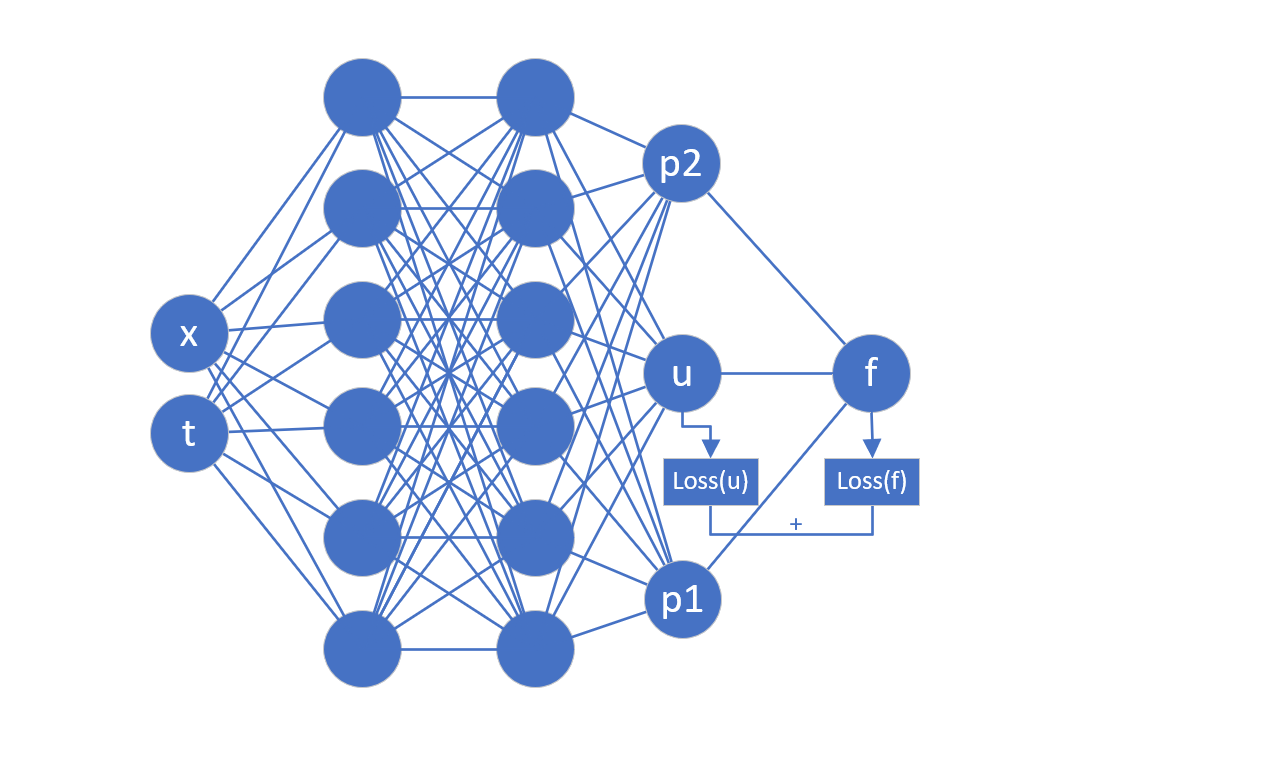
\includegraphics[width=12cm]{./imags/flower.png}
		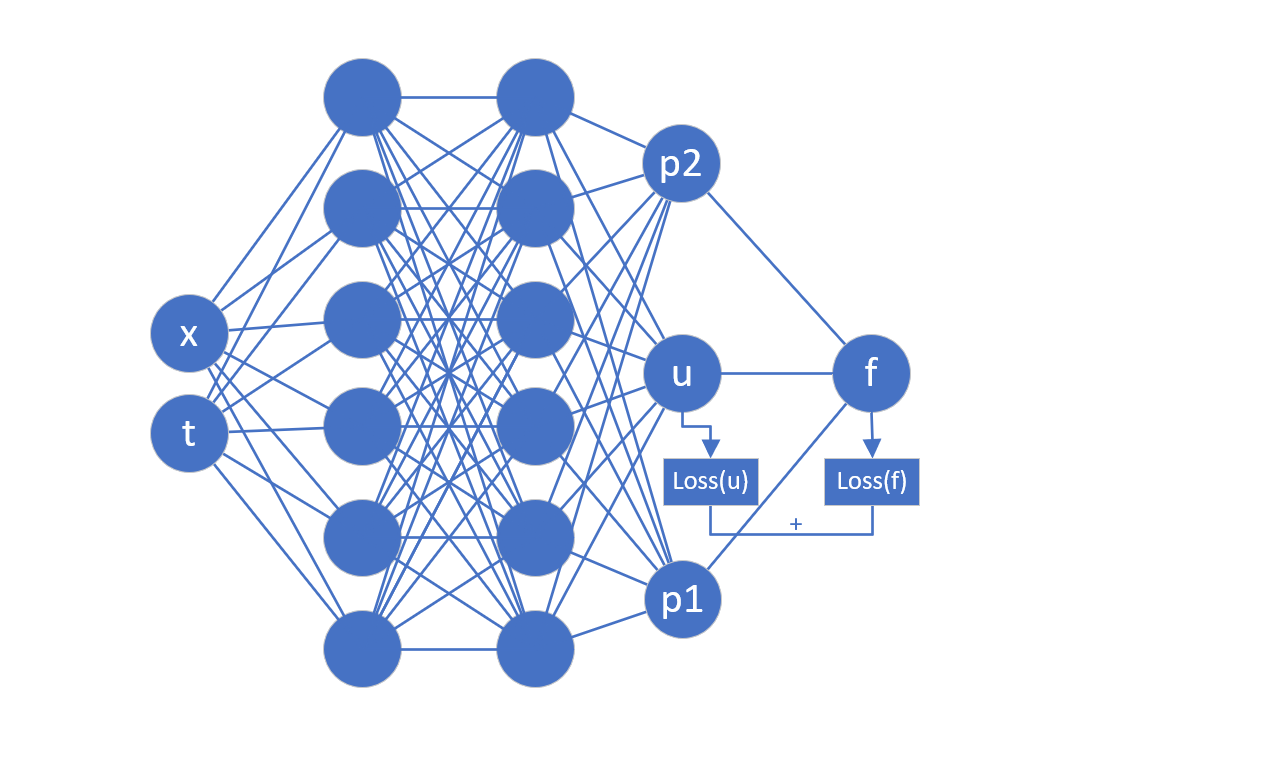
\includegraphics[height=10cm]{./imags/flower.png}
		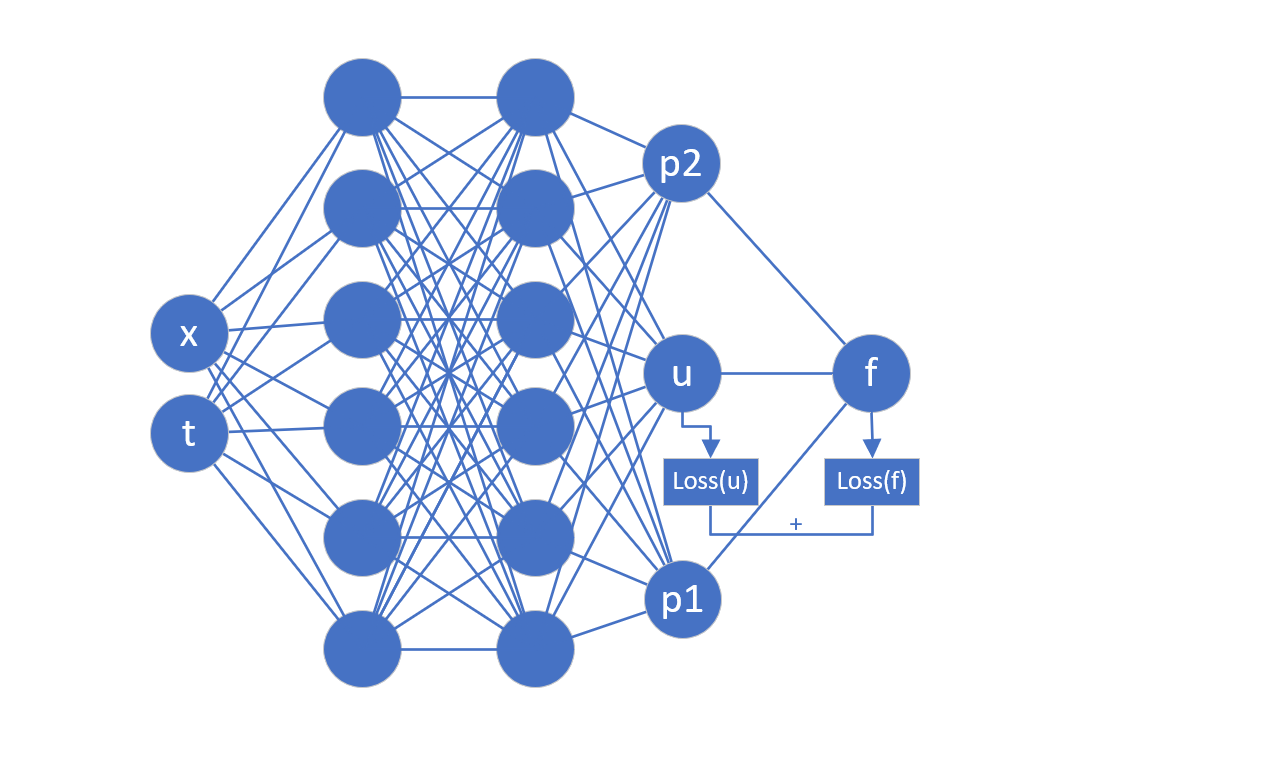
\includegraphics[scale=0.5]{./imags/flower.png}
		\caption{获得N的结构}
	\end{figure}
\end{frame}

\section{强调}
\begin{frame}{\secname}
	\begin{block}{多解性}
		反演的速度场具有唯一性吗?
	
		\qquad
	

		需要有合适的边界条件	
	\end{block}
	\begin{itemize}
		\item 只需要边界与初始位置的数据用于训练+正演算子正则化
		\begin{gather*}
			u \longrightarrow u(w,b)\\
			f \longrightarrow regulation (w,b)
		\end{gather*}

		\item 利用了自动微分的高精度
		\item 可以考虑加入权重系数平衡loss(u)和loss(f)。

	\end{itemize}
	\begin{enumerate}
		\item 1
	\end{enumerate}
\end{frame}

\section{页面布置}
\subsection{分两栏}
\begin{frame}{\secname}
	\begin{columns}
		\begin{column}{0.6\linewidth}
			\begin{itemize}
			\item 网络: 9 layers X 20 neurons 
			\item input 1: 输入x和t(边界条件与初始条件上随机),得到$u_{pred}$, 计算loss(u) 
			\item input 2: 输入x和t(全空间随机),得到$f_{pred}$, 计算 loss(f) 
			\item loss = loss(u)+loss(f)
			\end{itemize}
		\end{column}
		
		\begin{column}{0.45\linewidth}
			\begin{figure}[h]
				\centering
				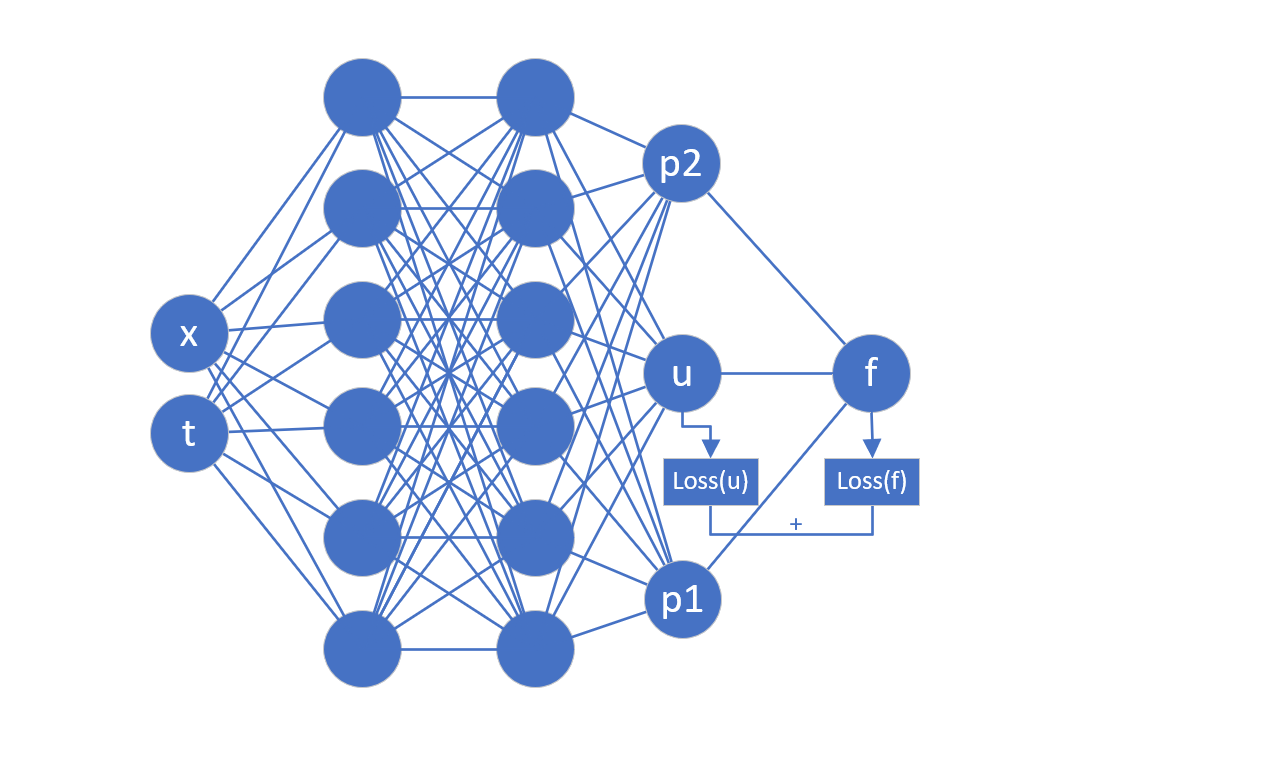
\includegraphics[width=5cm]{./imags/flower.png}
				\caption{加入正演算子的神经网络}
			\end{figure}
		\end{column}
	\end{columns}
\end{frame}
\subsection{空行}
\begin{frame}
	反演的速度场具有唯一性吗?
	
	\qquad
	
	\qquad
	

	需要有合适的边界条件
\end{frame}

\section{特效}
\subsection{动画}
\begin{frame}
	\begin{itemize}
		\item 1
		\item 2
		\pause
		\item 3
	\end{itemize}
\end{frame}

\end{document}
